\documentclass[letterpaper,12pt]{article}

\usepackage[scaled=0.92]{helvet}

\usepackage[colorlinks=true, linkcolor=blue]{hyperref}

\usepackage[english]{babel}
\selectlanguage{english}

\usepackage{microtype}
\usepackage{graphicx}
\usepackage{wrapfig}
\usepackage{enumitem}
\usepackage{amsmath}
\usepackage{index}
\usepackage[utf8]{inputenc}
\usepackage[svgnames]{xcolor}
\usepackage{url}
\usepackage{hyperref}
\usepackage{float}
\usepackage{longtable}
\usepackage[toc]{glossaries}
\usepackage{tabularx}

\begin{document}

\begin{titlepage}

\begin{center}
\vspace*{-1.2in}
\begin{figure}[htb]
\begin{center}

\includegraphics[width=10cm]{Concordia_logo.png}
\end{center}
\end{figure}
\begin{Large}
\vspace*{0.3in}
\textbf{Project Report} \\
\end{Large}
\vspace*{0.1in}
\begin{Large}
For\\
\end{Large}
\vspace*{0.1in}

\begin{Large}
\textbf{Deliverable 1} \\
\end{Large}
\vspace*{0.1in}

\begin{Large}
\textbf{METRICSTICS} \\
\end{Large}
\vspace*{0.3in}

\begin{large}
\textbf{Submitted By} \\
\vspace*{0.1in}
Amrinderpreet Singh\\
Anant Bir Singh\\
Gaganpreet Singh\\
Prabhjot Singh\\
Rahul Singh\\
Piyush Singla\\
\vspace*{0.2in}
\textbf{Submitted to}\\
\vspace*{0.1in}
Prof. Pankaj Kamthan\\
\vspace*{0.3in}

\begin{Large}
\textbf{SOEN 6611 - Software Measurement} \\
\vspace*{0.2in}
\textbf{Concordia University, Montreal, QC}
\end{Large}

\end{large}
\end{center}
\end{titlepage}


\newcommand{\CC}{C\nolinebreak\hspace{-.05em}\raisebox{.4ex}{\tiny\bf +}\nolinebreak\hspace{-.10em}\raisebox{.4ex}{\tiny\bf +}}
\def\CC{{C\nolinebreak[4]\hspace{-.05em}\raisebox{.4ex}{\tiny\bf ++}}}

\tableofcontents
\newpage
\section{Introduction}

\subsection{Scope}
In the ever-evolving landscape of data-driven decision-making within the software industry, there exists a pressing need for advanced software tools that can effectively cater to the intricate demands of software measurement. In this initial deliverable, we embark on a journey to conceptualize and develop METRICSTICS, an innovative software solution poised to address these needs. METRICSTICS aims to harness the power of descriptive statistics to empower professionals to analyze and interpret datasets comprehensively. Within this report, we will explore the foundational stages of METRICSTICS' development, including the establishment of critical Goal-Question-Metric (GQM) principles and the creation of a use case model for the system.

\subsection{Description}
METRICSTICS is envisioned to offer a comprehensive suite of statistical calculations and analyses:
\begin{enumerate}
\item Mean Calculation: METRICSTICS will calculate the arithmetic mean, providing a measure of central tendency for datasets.

\item Median Calculation: The system will determine the median, whether for datasets with odd or even numbers of elements, offering a robust representation of data distribution.

\item Mode Identification: METRICSTICS will identify modes, revealing the most frequently occurring values in a dataset.

\item Data Range: It will ascertain the minimum and maximum values within a dataset.

\item Variability Assessment: The system will calculate the standard deviation and mean absolute deviation, enabling software professionals to understand data variability and dispersion.
\end{enumerate}

\newpage
\section{PROBLEM 1: Goal-Question-Metric (GQM)}
We've applied the GQM approach to set a clear goal for METRICSTICS. We've formulated 12 specific questions and identified corresponding metrics to measure progress and performance.

\subsection{Goal}
Ensure the accuracy, usability, and user satisfaction of METRICSTICS to accommodate a wide range of scenarios.

\subsection{Questions and Metrics}
\begin{enumerate}
\item \textbf{Question:} How well does METRICSTICS handle increasingly large datasets?\\
\textbf{Metric:} Scalability Index, measuring METRICSTICS' performance as data size increases
\item \textbf{Question:} Is METRICSTICS able to identify multiple modes (o) when they exist in the dataset?\\
\textbf{Metric:} Count of identified modes and a list of mode values
\item \textbf{Question:} Does METRICSTICS consistently compute the median (d) accurately, especially for datasets with even n values?\\
\textbf{Metric:} Median Absolute Error (MedAE) for datasets with both odd and even n values
\item \textbf{Question:} Are users able to easily input their datasets into METRICSTICS?\\
\textbf{Metric:} Time taken for users to input a dataset and any input errors reported
\item \textbf{Question:} Does METRICSTICS provide consistent results when analyzing real and artificial data generated by a random data generator?\\
\textbf{Metric:} Comparative analysis of METRICSTICS results for real and generated datasets
\item \textbf{Question:} How intuitive is the process of obtaining descriptive statistics using METRICSTICS?\\
\textbf{Metric:} User satisfaction ratings for the intuitiveness of the interface\\
\\
\item \textbf{Question:} How effectively does METRICSTICS handle user data validation and error handling?\\
\textbf{Metric:} Number of errors encountered during data input and how they are handled
\item \textbf{Question:} How well does METRICSTICS perform when data is provided in different formats (e.g., integers, floating-point numbers)?\\
\textbf{Metric:} Accuracy of METRICSTICS across various data types
\item \textbf{Question:} Does METRICSTICS provide clear and understandable output of descriptive statistics?\\
\textbf{Metric:} Readability Score for METRICSTICS. It can be assessed using the Flesch-Kincaid Grade Level
\item \textbf{Question:} Does METRICSTICS consistently calculate the mean absolute deviation (MAD) accurately?\\
\textbf{Metric:} MAD Absolute Error (MADAE) for various datasets
\item \textbf{Question:} How consistent are the standard deviation ($\sigma$) calculations made by METRICSTICS across different datasets?\\
\textbf{Metric:} Standard Deviation Variability (SDV) across a range of datasets
\item \textbf{Question:} How well does METRICSTICS handle datasets with extreme outliers?\\
\textbf{Metric:} Robustness measure based on the impact of outliers on calculated statistics
\end{enumerate}
\newpage
\section{PROBLEM 2: Use Case Model}
\subsection{UML Use case Diagram}
\begin{figure}[htb]
\begin{center}
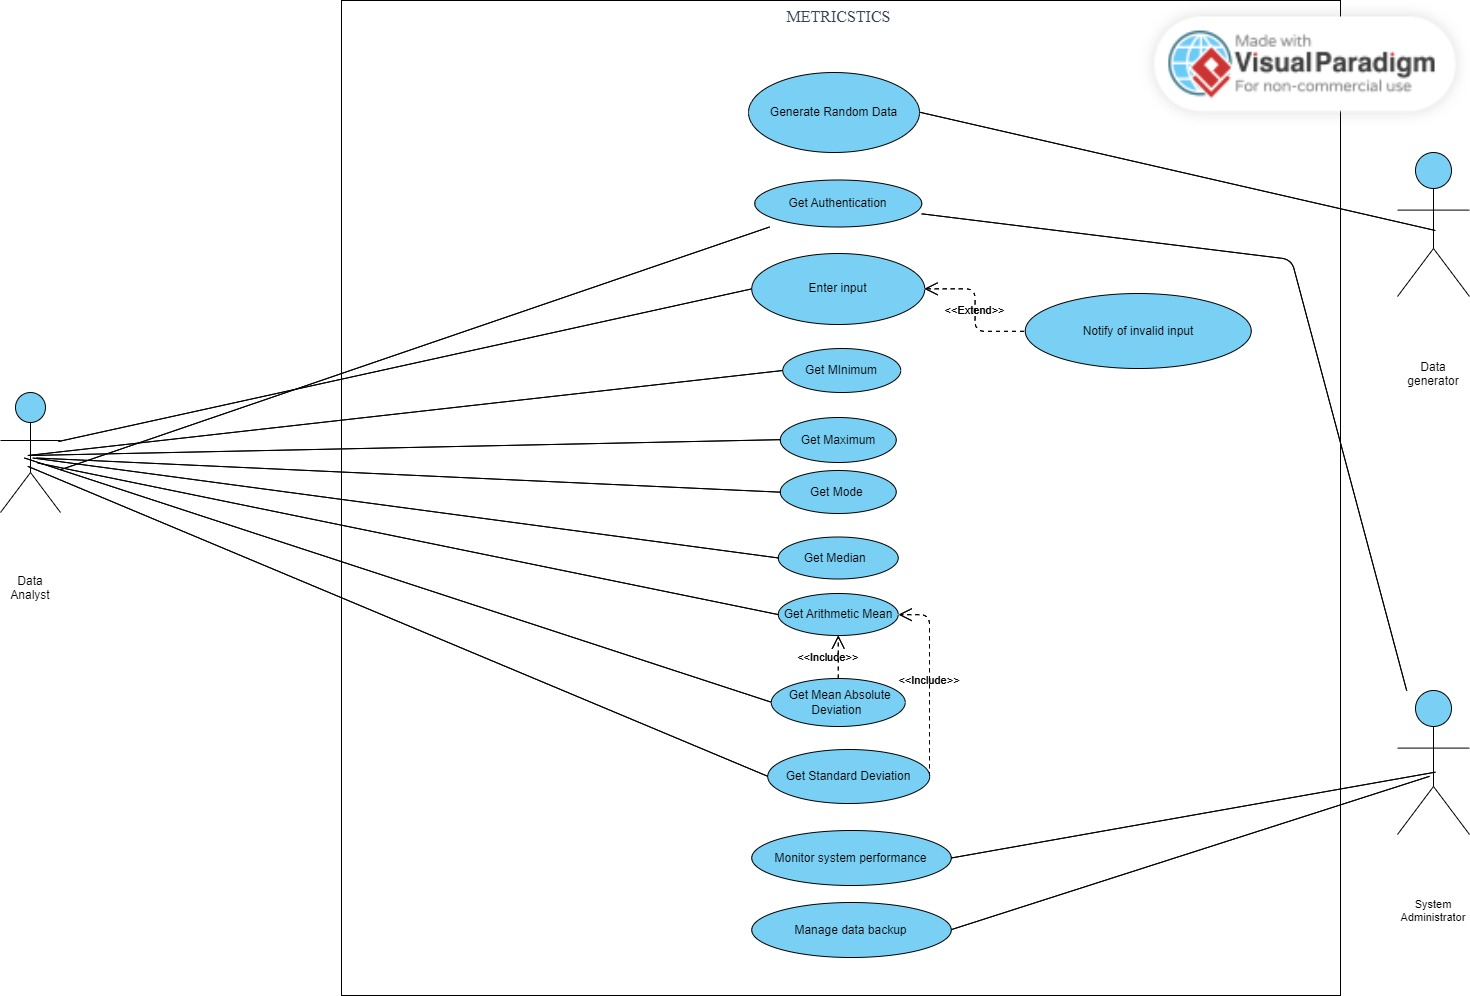
\includegraphics[width=14cm]{usecase.jpg}
\caption \protect UML Use Case Diagram of METRICSTICS
\end{center}
\end{figure}
\subsection {Actor and Use Case Descriptions}
\begin{itemize}
    \item \textbf {Actors:}
    \begin{itemize}
\item\textbf {Data Generator:} The Data Generator represents a system responsible for generating artificial and randomised datasets used for testing and evaluation within the METRICSTICS system.
\item\textbf {Data Analyst:} The Data Analyst actor represents users who input data, analyze it, and perform various statistical calculations to quantitatively describe a collection of data using METRICSTICS.
\item\textbf {System Administrator:} The System Administrator actor is responsible for overseeing and managing the overall system performance and maintenance tasks within METRICSTICS. 
\end{itemize}
    \item \textbf {Use Casses:}\\
\\
\begin{tabular}{|p{1.45in}|p{3.65in}|}
   \hline
    System & METRICSTICS \\
    \hline
    Identifier & UC-1 \\
    \hline
    Name & Generate Random Data \\
    \hline
    Pre-conditions & User launches the system\\
   \hline
    Post-conditions & Artificial dataset is fed to the system for analysis\\
   \hline
    Trigger & User selects the "Generate Random Data" option \\
    \hline
    Normal Scenario & The system generates an artificial dataset \\
    \hline
    Exceptional Scenario & None \\
    \hline
    Related Actor& Data Generator\\
    \hline
    Related Use Case & None\\
\hline
\end{tabular}\\
\bigskip
\bigskip

\begin{tabular}{|p{1.45in}|p{3.65in}|}
    \hline
    System & METRICSTICS \\
    \hline
    Identifier & UC-2 \\
    \hline
    Name & Get Authentication \\
    \hline
    Pre-conditions & User opens the METRICSTICS application\\
   \hline
    Post-conditions & User is successfully authenticated \\
   \hline
    Trigger & User launches the system \\
    \hline
    Normal Scenario &  \begin{itemize}
   \item User enters their credentials
   \item The system verifies the credentials
   \item If the credentials are valid, the user is granted access
   \end{itemize}\\
    \hline
    Exceptional Scenario & The system displays an error message \\
    \hline
    Related Actor& \begin{itemize}
   \item Data Analyst
   \item Data Administrator
   \end{itemize}\\
    \hline
    Related Use Case & None\\
\hline
\end{tabular}
\bigskip
\bigskip

\begin{tabular}{|p{1.45in}|p{3.65in}|}
    \hline
    System & METRICSTICS \\
    \hline
    Identifier & UC-3 \\
    \hline
    Name & Enter Input \\
    \hline
    Pre-conditions & User launches the system and logs in\\
   \hline
    Post-conditions & Data is successfully input, and statistics are calculated\\
   \hline
    Trigger & User selects the "Enter Input" option \\
    \hline
    Normal Scenario &  \begin{itemize}
   \item User inputs a dataset
   \item The system validates and processes the input
   \item Descriptive statistics are calculated
   \end{itemize}\\
    \hline
    Exceptional Scenario & The system notifies the Data Analyst of the invalid input \\
    \hline
    Related Actor& Data Analyst\\
    \hline
    Related Use Case & Notify of invalid input\\
\hline
\end{tabular}
\bigskip
\bigskip

\begin{tabular}{|p{1.45in}|p{3.65in}|}
    \hline
    System & METRICSTICS \\
    \hline
    Identifier & UC-4 \\
    \hline
    Name &  Get Minimum \\
    \hline
    Pre-conditions & User logs in and enters data\\
   \hline
    Post-conditions & Minimum value of the dataset is returned\\
   \hline
    Trigger & User selects the "Get Statistics" option \\
    \hline
    Normal Scenario &  \begin{itemize}
   \item User inputs a dataset
   \item The system calculates and returns the minimum value
   \end{itemize}\\
    \hline
    Exceptional Scenario & None \\
    \hline
    Related Actor& Data Analyst\\
    \hline
    Related Use Case & None\\
\hline
\end{tabular}
\bigskip
\bigskip

\begin{tabular}{|p{1.45in}|p{3.65in}|}
    \hline
    System & METRICSTICS \\
    \hline
    Identifier & UC-5 \\
    \hline
    Name &  Get Maximum \\
    \hline
    Pre-conditions & User logs in and enters data\\
   \hline
    Post-conditions & Maximum value of the dataset is returned\\
   \hline
    Trigger & User selects the "Get Statistics" option \\
    \hline
    Normal Scenario &  \begin{itemize}
   \item User inputs a dataset
   \item The system calculates and returns the maximum value
   \end{itemize}\\
    \hline
    Exceptional Scenario & None \\
    \hline
    Related Actor& Data Analyst\\
    \hline
    Related Use Case & None\\
\hline
\end{tabular}
\bigskip
\bigskip

\begin{tabular}{|p{1.45in}|p{3.65in}|}
    \hline
    System & METRICSTICS \\
    \hline
    Identifier & UC-6 \\
    \hline
    Name &  Get Mode \\
    \hline
    Pre-conditions & User logs in and enters data\\
   \hline
    Post-conditions & Mode (most frequent value) of the dataset is returned\\
   \hline
    Trigger & User selects the "Get Statistics" option \\
    \hline
    Normal Scenario &  \begin{itemize}
   \item User inputs a dataset
   \item The system calculates and returns the mode
   \end{itemize}\\
    \hline
    Exceptional Scenario & None \\
    \hline
    Related Actor& Data Analyst\\
    \hline
    Related Use Case & None\\
\hline
\end{tabular}
\bigskip
\bigskip

\begin{tabular}{|p{1.45in}|p{3.65in}|}
    \hline
    System & METRICSTICS \\
    \hline
    Identifier & UC-7 \\
    \hline
    Name &  Get Median \\
    \hline
    Pre-conditions & User logs in and enters data\\
   \hline
    Post-conditions & Median value of the dataset is returned\\
   \hline
    Trigger & User selects the "Get Statistics" option \\
    \hline
    Normal Scenario &  \begin{itemize}
   \item User inputs a dataset
   \item The system calculates and returns the median
   \end{itemize}\\
    \hline
    Exceptional Scenario & None \\
    \hline
    Related Actor& Data Analyst\\
    \hline
    Related Use Case & None\\
\hline
\end{tabular}
\bigskip
\bigskip

\begin{tabular}{|p{1.45in}|p{3.65in}|}
    \hline
    System & METRICSTICS \\
    \hline
    Identifier & UC-8 \\
    \hline
    Name & Get Arithmetic Mean \\
    \hline
    Pre-conditions & User logs in and enters data\\
   \hline
    Post-conditions & Arithmetic Mean (average) of the dataset is returned\\
   \hline
    Trigger & User selects the "Get Statistics" option \\
    \hline
    Normal Scenario &  \begin{itemize}
   \item User inputs a dataset
   \item The system calculates and returns the Arithmetic Mean
   \end{itemize}\\
    \hline
    Exceptional Scenario & None \\
    \hline
    Related Actor& Data Analyst\\
    \hline
    Related Use Case & \begin{itemize}
   \item Get Mean Absolute Deviation
   \item Get Standard Deviation
   \end{itemize}\\\\
\hline
\end{tabular}
\bigskip
\bigskip

\begin{tabular}{|p{1.45in}|p{3.65in}|}
    \hline
    System & METRICSTICS \\
    \hline
    Identifier & UC-9 \\
    \hline
    Name &  Get Mean Absolute Deviation \\
    \hline
    Pre-conditions & User logs in and enters data\\
   \hline
    Post-conditions & Mean absolute deviation of the dataset is returned\\
   \hline
    Trigger & User selects the "Get Statistics" option \\
    \hline
    Normal Scenario &  \begin{itemize}
   \item User inputs a dataset
   \item The system calculates and returns the Mean Absolute Deviation
   \end{itemize}\\
    \hline
    Exceptional Scenario & None \\
    \hline
    Related Actor& Data Analyst\\
    \hline
    Related Use Case & Get Arithmetic Mean \\
\hline
\end{tabular}
\bigskip
\bigskip

\begin{tabular}{|p{1.45in}|p{3.65in}|}
    \hline
    System & METRICSTICS \\
    \hline
    Identifier & UC-10 \\
    \hline
    Name &  Get Standard Deviation \\
    \hline
    Pre-conditions & User logs in and enters data\\
   \hline
    Post-conditions & Standard Deviation of the dataset is returned\\
   \hline
    Trigger & User selects the "Get Statistics" option \\
    \hline
    Normal Scenario &  \begin{itemize}
   \item User inputs a dataset
   \item The system calculates and returns the Standard Deviation
   \end{itemize}\\
    \hline
    Exceptional Scenario & None \\
    \hline
    Related Actor& Data Analyst\\
    \hline
    Related Use Case & Get Arithmetic Mean \\
\hline
\end{tabular}
\bigskip
\bigskip

\begin{tabular}{|p{1.45in}|p{3.65in}|}
    \hline
    System & METRICSTICS \\
    \hline
    Identifier & UC-11 \\
    \hline
    Name &  Monitor System Performance \\
    \hline
    Pre-conditions & System Administrator launches the system\\
   \hline
    Post-conditions & System performance metrics are monitored\\
   \hline
    Trigger &  System Administrator selects the "View System Performance" option \\
    \hline
    Normal Scenario & System Administrator monitors system performance metrics in real-time \\
    \hline
    Exceptional Scenario & None \\
    \hline
    Related Actor& System Administrator\\
    \hline
    Related Use Case & None \\
\hline
\end{tabular}
\bigskip
\bigskip

\begin{tabular}{|p{1.45in}|p{3.65in}|}
    \hline
    System & METRICSTICS \\
    \hline
    Identifier & UC-12 \\
    \hline
    Name & Manage Data Backup \\
    \hline
    Pre-conditions & System Administrator launches the system\\
   \hline
    Post-conditions & Data backup procedures are initiated and completed\\
   \hline
    Trigger & System Administrator selects the "Manage Data Backup" option \\
    \hline
    Normal Scenario & System Administrator initiates data backup and completes it \\
    \hline
    Exceptional Scenario & None \\
    \hline
    Related Actor& System Administrator\\
    \hline
    Related Use Case & None \\
\hline
\end{tabular}
\end{itemize}
\section {Version Control}
You can access the GitHub repository at:\\
\href{https://github.com/theOGCodeWitcher/SOEN-6611-METRICSTICS}{https://github.com/theOGCodeWitcher/SOEN-6611-METRICSTICS}
\section{References}
\textit{https://users.encs.concordia.ca/~kamthan/courses/soen-6611} \\
\textit{https://www.visual-paradigm.com/} \\
\textit{https://chat.openai.com/}
\end{document}
